\documentclass[11pt]{article}
\usepackage{bookmark}
\usepackage{algorithm}
\usepackage{algpseudocode}
\usepackage{amsfonts}
\usepackage{amsmath}
\usepackage{amssymb}
\usepackage{amsthm}
\usepackage{bm}
\usepackage{color}
\usepackage{comment}
\usepackage{float}
\usepackage{graphicx}
%\usepackage[hidelinks]{hyperref}
\usepackage{makecell}
\usepackage[caption=false,font=footnotesize,subrefformat=parens,labelformat=parens]{subfig}
\usepackage{wrapfig}
\usepackage{url}
\usepackage[table]{xcolor}
%
\setlength{\parindent}{0.25in}
\setlength{\parskip}{.05in}
\pagestyle{plain}
%Title, date an author of the document
\title{Literature Review}
\author{Bardia Mojra}


\begin{document}
\maketitle
\thispagestyle{empty}
\begin{center}
      Robotic Vision Lab
\end{center}

\begin{center}
      The University of Texas at Arlington
\end{center}
\bigskip
\bigskip
\begin{center}
{\Large Reinforcement Learning of Active Vision for Manipulating Objects under
Occlusions}
\end{center}

\section{Metadata}
\begin{itemize}
      \item Authors: Ricson Cheng, Arpit Agarwal, Katerina Fragkiadaki
      \item Code: \url{https://github.com/ricsonc/ActiveVisionManipulation}
      \item Paper: \url{https://arxiv.org/pdf/1811.08067.pdf}
\end{itemize}

\section{Introduction}
\par In this paper, the authors propose a novel reinforcement learning method
for monocular RGB grasping systems where camera pose is controlled through
visual feedback to reduce occlusions. The task of simple object grasping has been fairly achieved
but in the real world, there are often occlusions with other objects that needs .
First, the authors pose the question of learning manipulation policies under
occlusions and propose agents capable of hand-eye movement coordination with
various distractors present in the scene. Secondly, they introduce a \textbf{modular
actor-critic network architecture} based on \cite{andrychowicz2017hindsight}
for active perception and action in Mujoco simulation environment, \cite{todorov2012mujoco}.
This paper examines various reinforcement learning modalities and highlights the
importance of environment difficulty (distractors) in \textbf{curriculum learning}
methods.

\section{Problem Statement}
\par The authors focus on the task of pushing an object to target locations in
environments with distractors where an actor-critic architecture is deployed for
eye-hand coordination. Hand-eye or camera-griper coordination is base on
\cite{soatto2013actionable} and by integrating it, the authors, aim to achieve
state estimation easier (train faster) by reducing an \textbf{information gap}
or deficiency caused by static camera. First, they trained a vanilla CNN for the
task of pushing an object with minimal distractors present, which failed. Then
they integrated an object detector module in the actor-critic architecture which
enabled effective learning. Secondly, they trained state-of-the-art reinforcement
learning models with simple distractors present and occasionally occluded the
target object, which also failed to learn. Then, they initialized the actor-critic
network weights from policies learned in environments without distractors. This
reinforces what is hypothesized by \textit{curriculum learning}.

\section{Method}
The authors represent the mentioned problem in form a multi-goal Partially
Observable Markov Decision Process (POMDP) which is a constraint satisfaction
problem formulation. The reinforcement learning environment is modelled by the
observations ($\mathcal{O}$), states ($\mathcal{S}$), goals ($\mathcal{G}$),
gripper actions ($\mathcal{A^G}$) and camera actions ($\mathcal{A^C}$) spaces.

The critic network (a CNN) take RGB images as input and encodes low dimensional
embeddings using what-where decomposition which is presents object appearances
$f_t$.
Moreover, a faster-RCNN \cite{ren2015faster} is used for object detection,
followed by PnP for target object pose estimation, $\hat{o_t}$.

The authors use HER's \cite{andrychowicz2017hindsight} object-centric
representation as it is shown to result in faster learning based on empirical
data. HER also introduces the powerful idea of learning from failed experiences
are encoded and stored in an \textbf{experience buffer} to draw heuristics from
in possible future states. This allows the agent to extract much greater level
of information from previously seen data.

\section{Experiments}

\begin{center}
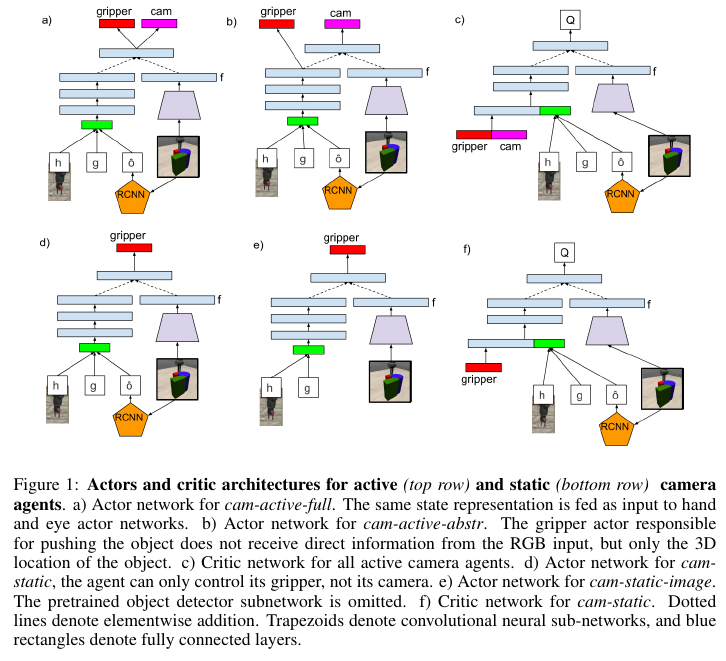
\includegraphics[scale=.4]{fig01}

\bigskip

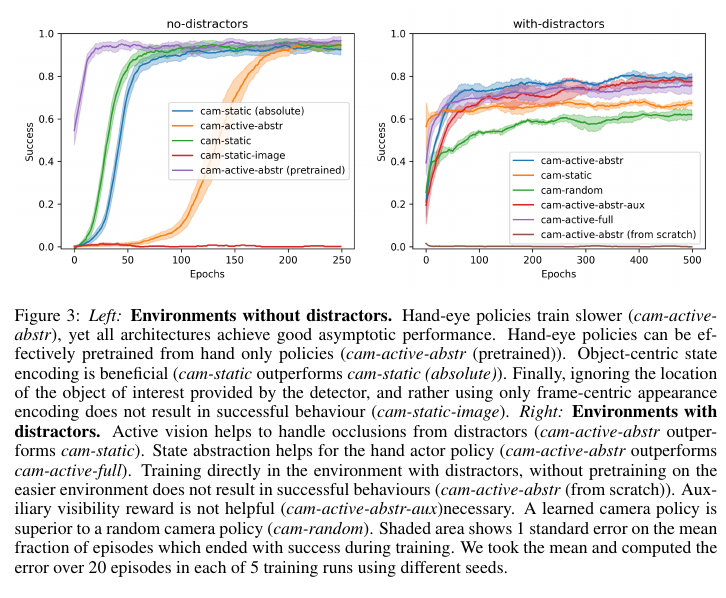
\includegraphics[scale=.4]{fig03}
\end{center}


%Sets the bibliography style to UNSRT and import the
%\newpage
\bibliography{references}
\bibliographystyle{ieeetr}

\end{document}
